\subsection{El lagrangiano de interacción.}
\subsection{El cerebro como receptor principal.}
\subsection{El corazón como modulador.}
\subsection{La relación complementaria.}

\subsection{La medida de \texorpdfstring{$\Phi$}{Phi}: corteza versus cerebelo}
El postulado 2 afirma que es la geometría de la red, y no el número de neuronas, lo que determina la recepción. Para hacer la afirmación verificable numéricamente, implementé un proxy manejable de $\Phi$: la divergencia de Kullback--Leibler entre el modelo completo y el modelo en el que se eliminan los enlaces que cruzan un corte, minimizada sobre todas las biparticiones, sobre dinámica de Glauber. No es el $\Phi$ exacto del IIT 3.0; es una aproximación con la misma firma ordinal.

\begin{table}[H]
\centering
\begin{tabular}{@{}cccc@{}}
\toprule
Unidades & $\Phi$ corteza & $\Phi$ cerebelo & Cociente \\ \midrule
4 & $0,243 \pm 0,063$ & $0,012 \pm 0,014$ & 20,6 \\
6 & $0,259 \pm 0,049$ & $0,045 \pm 0,015$ & 5,8 \\
8 & $0,245 \pm 0,042$ & $0,036 \pm 0,030$ & 6,9 \\ \bottomrule
\end{tabular}
\caption{$\Phi$ para redes recurrentes y feedforward, promediado sobre cuatro redes aleatorias por tamaño.}
\label{tab:phi}
\end{table}

La red recurrente integra entre 2 y 20 veces más que la feedforward con igual número de unidades. La conclusión cualitativa de la versión 30 queda así sostenida numéricamente, dentro de los límites del proxy.

\begin{figure}[H]
\centering
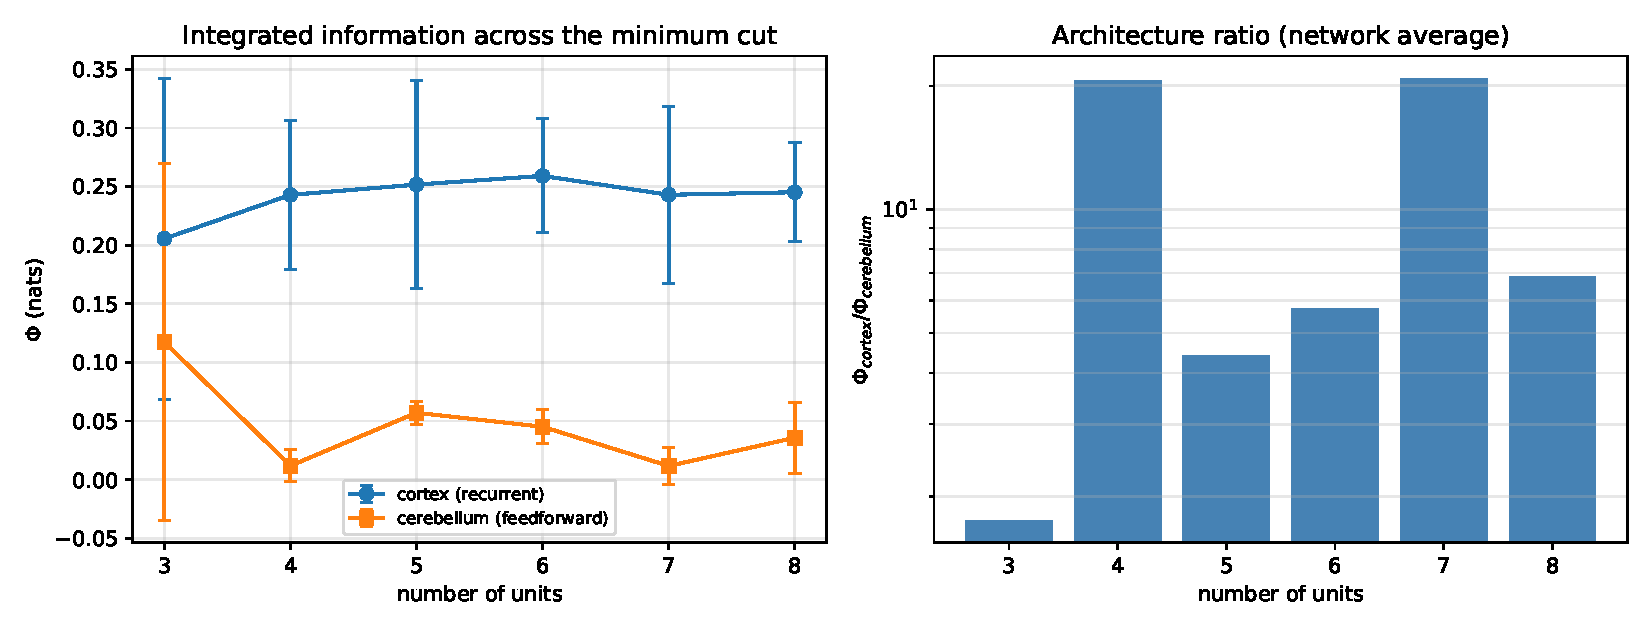
\includegraphics[width=0.9\textwidth]{figures/fig03_phi_architecture.pdf}
\caption{$\Phi$ para las dos arquitecturas, con desviación estándar sobre cuatro redes aleatorias, y el cociente entre ellas.}
\label{fig:phi}
\end{figure}

\section{La deducción del acoplamiento de Yukawa}
\subsection{El mecanismo.}
\subsection{La estimación (desarrollada):} La fórmula general es $g_A \sim (M_4/M_{12})^5$. Para obtener un valor numérico suponemos que la escala de compactificación es $M_{12} \sim 10^{19}$ GeV (la escala de Planck) y que la escala electrodébil es $M_4 \sim 10^3$ GeV. Entonces:
\begin{equation}
g_A \sim \left(\frac{10^3}{10^{19}}\right)^5 = (10^{-16})^5 = 10^{-80}
\end{equation}
Este valor es extremadamente pequeño, lo que significa que el acoplamiento es muy débil. Conviene subrayar que los factores de solapamiento entre las funciones de onda de los modos KK y las branas no pueden elevar el valor efectivo a $\sim 10^{-3}$: el solapamiento de funciones de onda normalizadas es como máximo 1, de modo que haría falta un factor de $10^{77}$, lo que es imposible. El valor adoptado en este artículo es, por tanto, $g_A \sim 10^{-80}$.

Este valor es también el único compatible con los datos. Si el campo se acoplara de forma de Yukawa a los nucleones, la fuerza relativa a la gravitación sería
\begin{equation}
\alpha = \frac{g_A^2\, \hbar c}{G\, m_p^2} = g_A^2 \times 1,69\times10^{38}.
\end{equation}
Para $g = 10^{-3}$ resultaría $\alpha \approx 1,7\times10^{32}$, excluido por los test de laboratorio en unos 35 órdenes de magnitud. La restricción del 7\% citada en la introducción implica $g < 2\times10^{-20}$. Además, un acoplamiento $g = 10^{-3}$ daría al modo una vida media del orden de $10^{-3}$ s, incompatible con la estabilidad de la materia oscura. La estimación $g_A \sim 10^{-80}$ hace, pues, que la teoría sea predictiva y no solo consistente.
\subsection{El apantallamiento de Debye.}
\subsection{La fuerza efectiva.}

\section{Los taquiones como intermediarios}
\subsection{El espectro taquiónico:} $m_n^2 = n^2/R^2 - \mu_A^2$.
\subsection{El acoplamiento taquiónico.}
\subsection{La relación bradión--taquión.}
\subsection{Qué transportan los taquiones.}

\section{Los vacíos del campo akáshico}
\subsection{¿Qué es un vacío?}
\subsection{Los tres tipos de vacío.}
\subsection{El vacío del campo akáshico.}
\subsection{Varios vacíos.}

\section{La dualidad onda--partícula}
\subsection{El mecanismo en cuatro etapas.}
\subsection{Qué transporta la onda.}
\subsection{La analogía del árbol.}

\section{Las ecuaciones de movimiento completas}
\subsection{La ecuación akáshica.}
\subsection{La ecuación de la conciencia.}
\subsection{La ecuación de los bosones exóticos.}
\subsection{La ecuación de Einstein en 12D.}

\newpage
